soi%\documentclass{llncs}

%\usepackage{graphicx}
%\usepackage{pifont}
%\usepackage{amsmath,amssymb}
%\usepackage[english]{babel}
%\usepackage[utf8]{inputenc}
%\usepackage[ruled,vlined]{algorithm2e}
%\usepackage{hyperref}
%\usepackage{float} 
%\usepackage{multirow} 
%\usepackage{booktabs}
%\usepackage[disable]{todonotes}
%\usepackage{todonotes}
%\usepackage{mdframed}
%\usepackage{wrapfig}
%\usepackage{booktabs}
%\usepackage{cha333:tabulary}
%\usepackage{caption}
%\usepackage{comment}
%\usepackage{tikz}
%\usepackage{xspace}
%\usepackage{times}
%\usepackage{subfigure}

%\newcommand{\haken}{{\ding{51}}}
%\newcommand*\rot{\rotatebox{87}}



%\begin{document}

\chapter{Evaluating Entity Annotators Using GERBIL}

%\author{
%Ricardo Usbeck \and 
%Michael Röder \and
%Axel-Cyrille Ngonga Ngomo
%}

%\institute{
%University of Leipzig, Germany\\\email{\{usbeck,roeder,ngonga\}@informatik.uni-leipzig.de}
%}

%\maketitle

%\begin{abstract}
The need to bridge between the unstructured data on the Document Web and the structured data on the Web of Data has led to the development of a considerable number of annotation tools. However, these tools are hard to compare due to the diversity of data sets and measures used for evaluation. 
We will demonstrate GERBIL, an evaluation framework for semantic entity annotation that provides developers, end users and researchers with easy-to-use interfaces for the agile, fine-grained and uniform evaluation of annotation tools on 11 different data sets within 6 different experimental settings on 6 different measures. 
%We present the different types of experiments as well as the human-readable and machine-readable output formats supported by GERBIL. In addition, we show how the permanent experiment URIs provided by GERBIL ensure the reproducibility and archiving of evaluation results. Finally, we show how GERBIL can provide developers with diagnostics that allow to spot current strengths and weaknesses of their annotators. 
%\end{abstract}


\section{Introduction}
%The implementation of the original vision behind the Semantic Web demands the development of approaches and frameworks for the seamless extraction of structured data from text. 
The need for extracting structured data from text has led to the development of a large number of tools dedicated to the extraction of structured data from unstructured data (see~\cite{GERBIL} for an overview).
% \cite{TagMe2,AIDA,spotlight,milne2008learning,babelfy,piccinno2014tagme,rizzo2014,Steinmetz2013,AGDISTIS_ISWC}. Still, the provision of comparable results for these tools remains a tedious problem. 
%The issue of  comparability of results is not to be regarded as being intrinsic to the annotation task.% Indeed, it is now well established that scientists spend between 60 and 80\% of their time preparing data for experiments \cite{GIL2014,jermyn1999preparing,peng2011reproducible}.
%Data preparation being such a tedious problem in the annotation domain is mostly due to the different formats of the gold standards as well as the different data representations across reference data sets.
%
%These restrictions have led to authors evaluating their approaches on data sets (1) that are available to them and (2) for which writing a parser as well as of an evaluation tool can be carried out with reasonable effort.
%In addition, a large number of quality measures have been developed and used actively across the annotation research community to evaluate the same task, leading to the results across publications on the same topics not being easily comparable. For example, while some authors publish macro-F-measures and simply call them F-measures, others publish micro-F-measures for the same purpose, leading to significant discrepancies across the scores. The same holds for the evaluation of how well entities match. Indeed, partial matches and complete matches have been used in previous evaluations of annotation tools \cite{Cornolti,fox}. This heterogeneous landscape of tools, data sets and measures leads to a poor repeatability of experiments, which makes the evaluation of the real performance of novel approaches against the state of the art rather difficult.
%Recently, various benchmarking framework for entity annotation systems occurred focusing on different aspects.
%The BAT-framework~\cite{Cornolti} is designed to facilitate the benchmarking of named entity recognition (NER), named entity disambiguation (NED) and concept tagging approaches.
%BAT compares seven existing entity annotation approaches using Wikipedia as reference, and offers six different task types, five different matchings and six evaluation measures providing five data sets.
%Rizzo et al.~\cite{rizzo2014} present a state-of-the-art study of NER and NEL systems for annotating newswire and micropost.
In this demo, we present GERBIL, a framework for the evaluation of entity annotation frameworks. GERBIL provides a GUI that allows (1) configuring and running experiments, (2) assigning persistent URLs to experiments (better reproducibility and archiving), (3) exporting the results of the experiments in human- and machine-readable formats as well as (4) displaying the results w.r.t. the data sets and the features of the data sets on which the experiments were performed. %By these means, GERBIL goes beyond the state of the art by extending the BAT-framework~\cite{Cornolti} as well as~\cite{rizzo2014} in several dimensions to enhance reproducibility, diagnostics and publishability of the results  of entity annotation systems. 

%In this paper, we present GERBIL -- a general entity annotator benchmark --, a community-driven effort to enable the continuous evaluation of annotation tools. 
GERBIL is an open-source and extensible framework that allows evaluating tools against (currently) \overallGERBILannotators different annotators on \overalldatasets different data sets within 6 different experiment types. 
%By integrating such a large number of data sets, experiment types and frameworks, GERBIL allows users to evaluate their tools against other semantic entity annotation systems (short: entity annotation systems) by using exactly the same setting, leading to fair comparisons based on exactly the same measures. 
%While the evaluation core of GERBIL is based on the BAT-framework \cite{Cornolti}, our approach goes beyond the state of the art in several respects:
%\begin{itemize}
%\item GERBIL provides \emph{persistent URLs} for experimental settings. Hence, by using GERBIL for experiments, tool developers can ensure that the settings for their experiments (measures, data sets, versions of the reference frameworks, etc.) can be reconstructed in a  unique manner in future works. 
%\item Through experiment URLs, GERBIL also addresses the problem of \emph{archiving} experimental results and allows end users to gather all pieces of information required to choose annotation frameworks for practical applications.
%\item GERBIL aims to be a \emph{central repository for annotation results} without being a central point of failure: While we make experiment URLs available, we also provide users directly with their results to ensure that they use them locally without having to rely on GERBIL.
%\item The results of GERBIL are published in a \emph{machine-readable format}. In particular, our use of DataID~\cite{dataID} to denote tools and data sets ensures that results can be easily combined and queried (for example to study the evolution of the performance of frameworks) while the exact configuration of the experiments remains uniquely reconstructable. By these means, we also tackle the problem of \emph{reproducibility}. 
%\item Through the provision of results on different data sets of different types and the provision of results on a simple user interface, GERBIL also provides means to quickly gain an overview of the current performance of annotation tools, thus providing (1) developers with insights pertaining to the type of data on which their accuracy needs improvement and (2) end users with insights allowing them to choose the right tool for the tasks at hand.
%\item With GERBIL we introduce the notion of knowledge base-agnostic benchmarking of entity annotation systems through generalized experiment types. By these means, we allow benchmarking tools against reference data sets from any domain grounded in any reference knowledge base. 
%\end{itemize}
To ensure that our framework is useful to both end users and tool developers, its architecture and interface were designed to allow (1) the easy integration of annotators through REST services, (2) the easy integration of data sets via DataHub\footnote{\url{http://datahub.io}}, file uploads or direct source code integration, (3) the addition of new performance measures, (4) the provision of diagnostics for tool developers and (5) the portability of results. 
%\begin{itemize}
%\item \textbf{Easy integration of annotators}: We provide a wrapping interface that allows annotators to be evaluated via their REST interface. In particular, we integrated \numberOfadditionalAnnotators additional annotators not evaluated against each other in previous works (e.g., \cite{Cornolti}).  
%\item \textbf{Easy integration of data sets}: We also provide means to gather data sets for evaluation directly from data services such as DataHub.\footnote{\url{http://datahub.io}} In particular, we added \numberOfadditionaldata sets new data sets to GERBIL.
%\item \textbf{Easy addition of new measures}: The evaluation measures used by GERBIL are implemented as interfaces. Thus, the framework can be easily extended with novel measures devised by the annotation community.
%\item \textbf{Extensibility}: GERBIL is provided as an open-source platform\footnote{Available at \url{http://gerbil.aksw.org}.} that can be extended by members of the community both to new tasks and different purposes.
%\item \textbf{Diagnostics}: The interface of the tool was designed to provide developers with means to easily detect aspects in which their tool(s) need(s) to be improved. 
%\item \textbf{Portability of results}: We generate human- and machine-readable results to ensure maximum usefulness and portability of the results generated by our framework. 
%\end{itemize}
%\todo[inline]{summarize rest}
More information on GERBIL as well as a link to the online demo can be found at the project webpage at \url{http://gerbil.aksw.org}.
%and at the code repository page \url{https://github.com/AKSW/gerbil}
%The online version of this demo can be accessed at \url{http://gerbil.aksw.org/gerbil}. 
%This paper is a demo paper to the WWW 2015 paper \cite{GERBIL}.

%\todo[inline]{What will be shown in the demo?}
\section{GERBIL in a nutshell}
\label{cha333:sec:architecture}
\begin{figure}[tb]
\centering
%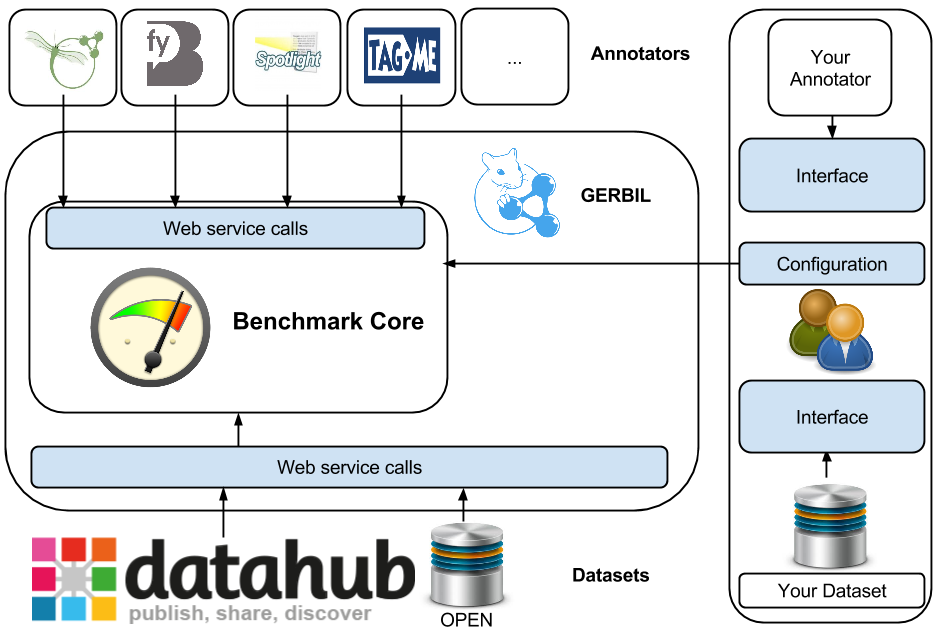
\includegraphics[width=\linewidth]{GERBIL_new_architectur}
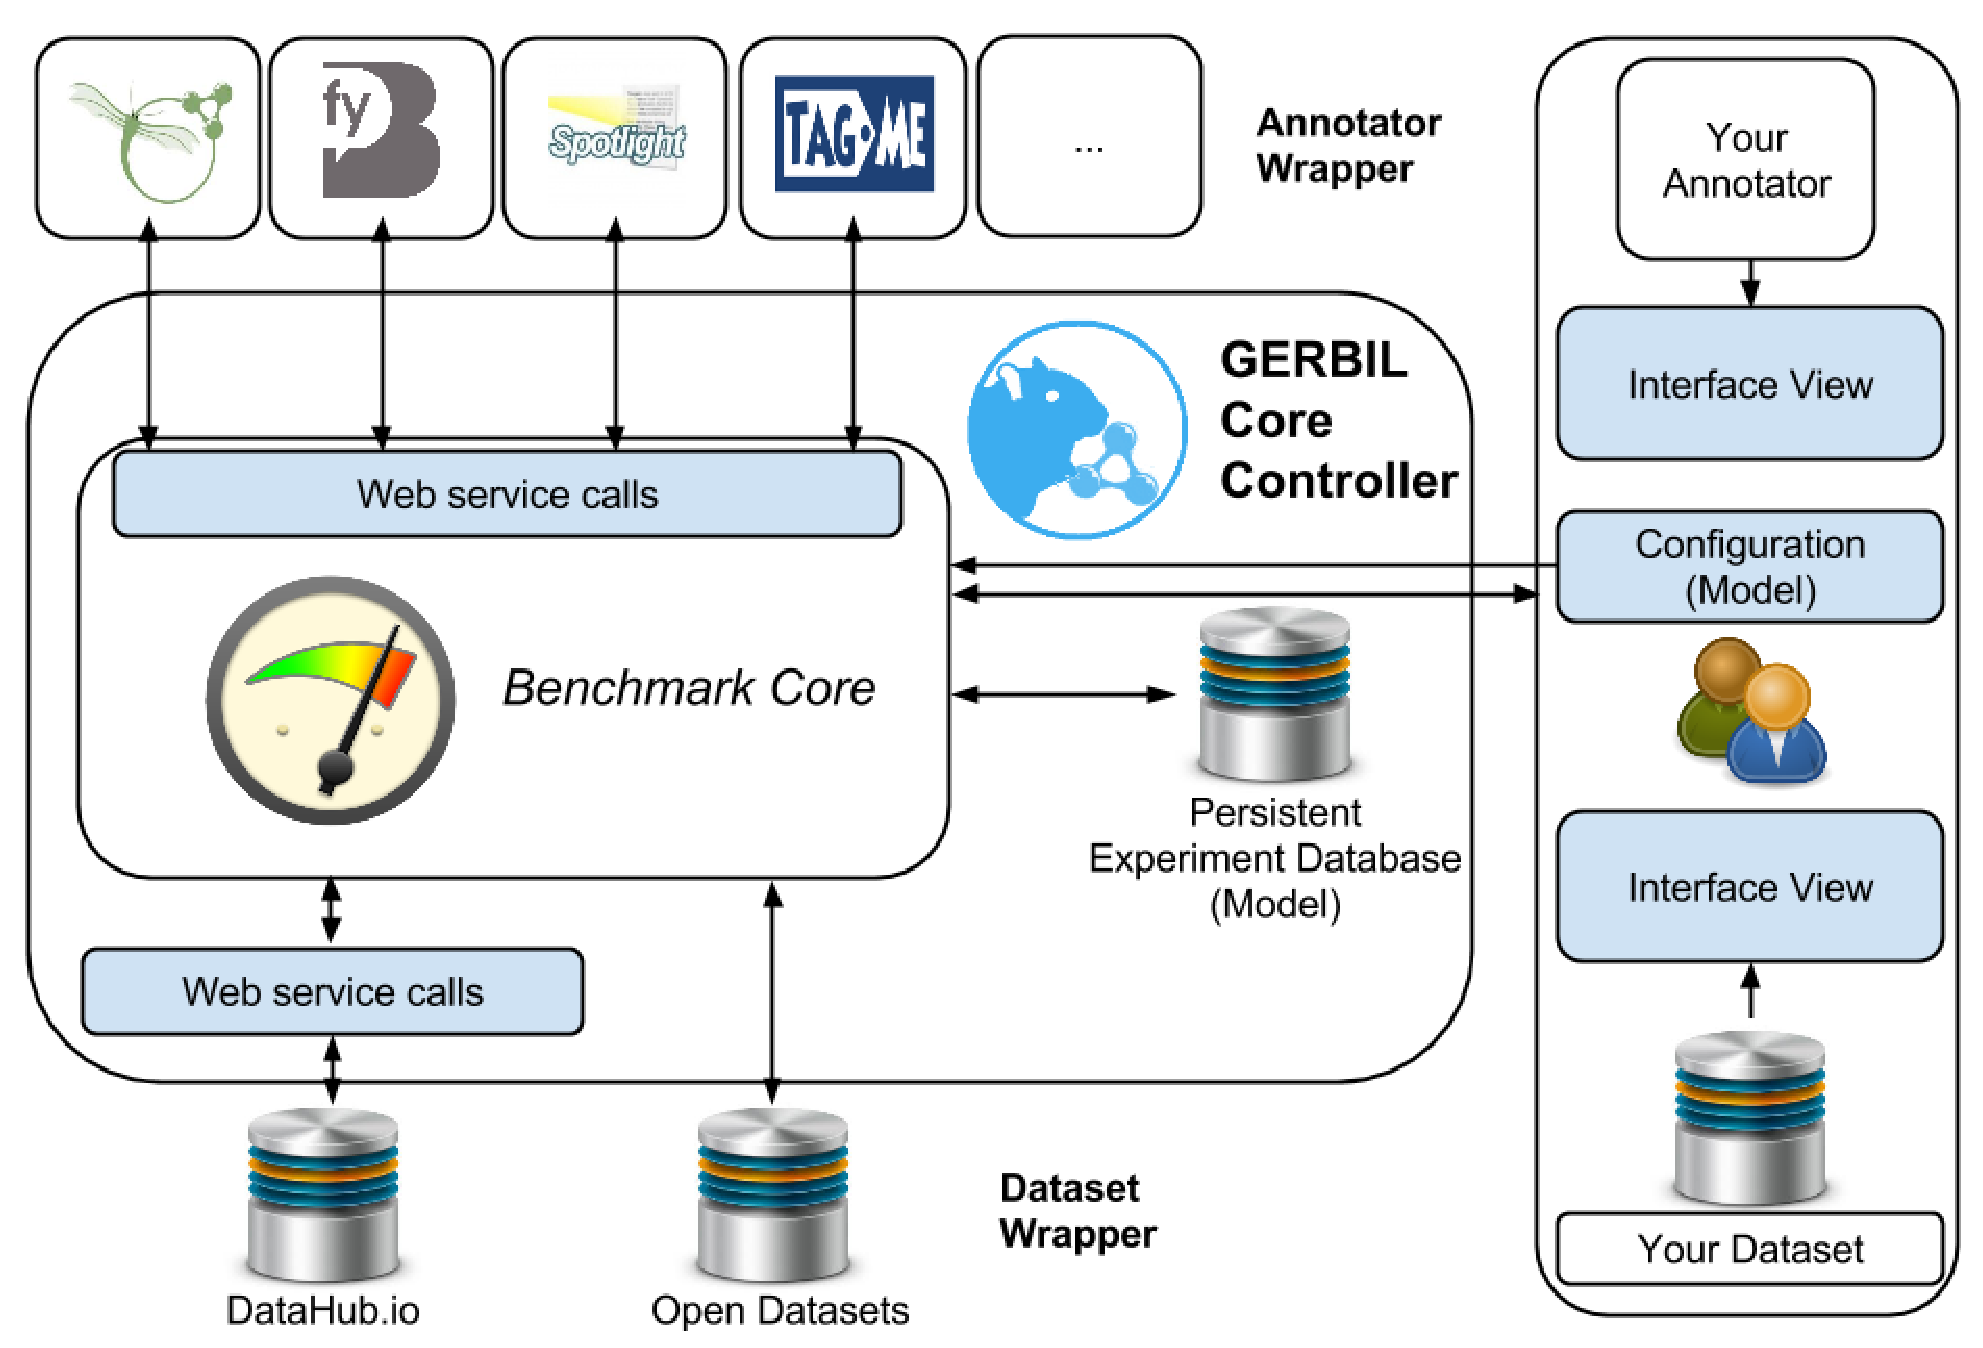
\includegraphics[width=0.7\linewidth]{part_02/benchmarking/ESWC_GERBIL_demo/gerbiloverview.eps}
%\vspace{-5mm}
\caption{Overview of GERBIL's abstract architecture. Interfaces to users and providers of data sets and annotators are marked in blue.
}
\label{cha333:fig:architecture}
%\vspace{-2mm}
\end{figure}

An overview of GERBIL's architecture is given in Figure~\ref{cha333:fig:architecture}. 
Based on this architecture, we will explain the features that we will present in the demonstration of the GERBIL framework.
%All features will be presented through the online demo at \url{http://gerbil.aksw.org/gerbil}.

\begin{figure}[htb]
\centering
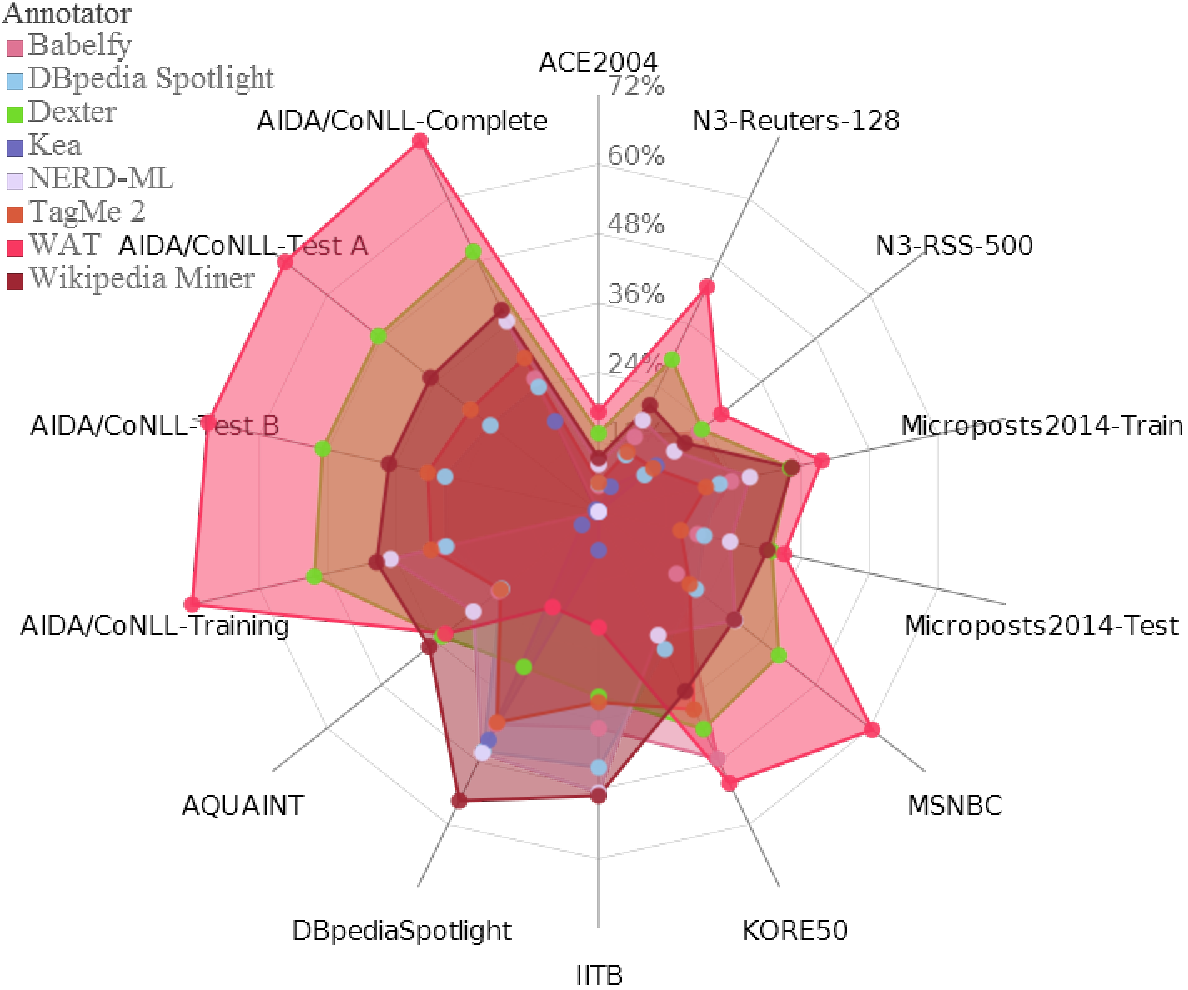
\includegraphics[width=\textwidth]{part_02/benchmarking/ESWC_GERBIL_demo/results.pdf}
\caption{Example spider diagram of recent A2KB experiments with weak annotation matching.}
\label{cha333:fig:spiderfmeasure}
\end{figure}

\begin{figure}[htb]
\centering
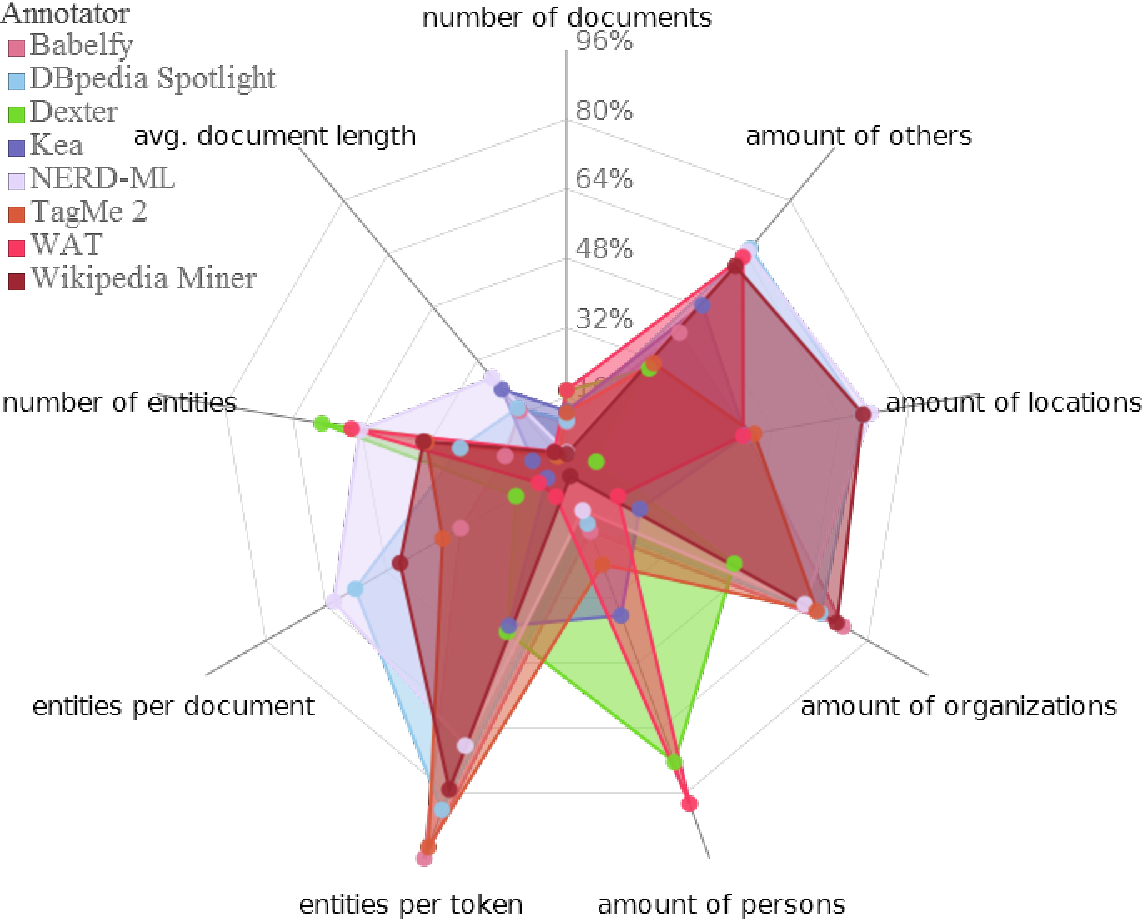
\includegraphics[width=\textwidth]{part_02/benchmarking/ESWC_GERBIL_demo/correlations.pdf}
\caption{Spider diagram of correlations between annotation results and data set features.}
\label{cha333:fig:spiderfeature}
\end{figure}


\begin{wrapfigure}{l}{6cm}
\centering
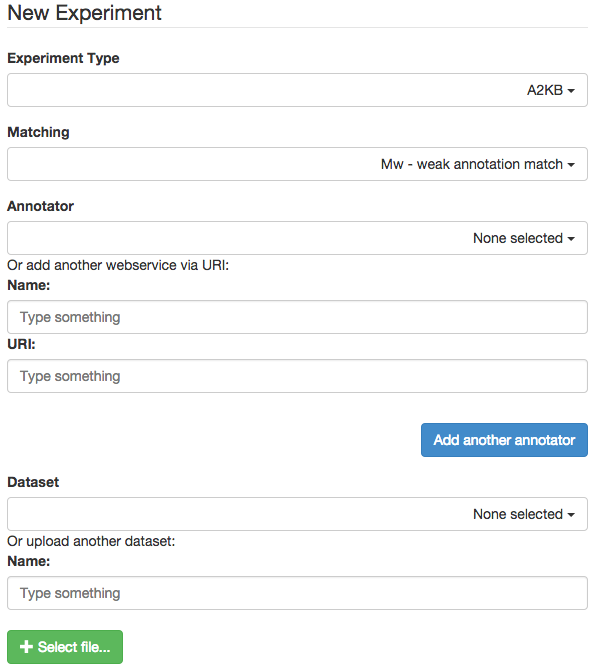
\includegraphics[width=0.95\linewidth]{part_02/benchmarking/ESWC_GERBIL_demo/screenshot}
\caption{Experiment configuration screen.}
\label{cha333:fig:screenshot}
\end{wrapfigure}

\textbf{Feature 1: Experiment types.}
An experiment type defines the way used to solve a certain problem when extracting information.
GERBIL extends the six experiments types provided by the BAT framework~\cite{cornolti} (including entity recognition and disambiguation). 
%and extends them by the idea to not only link to Wikipedia but to any knowledge base $K$, see~\cite{GERBIL}.
%The six experiment types implemented in GERBIL are (1) \emph{D2KB}, i.e., disambiguating a set of \emph{given} entity mentions to entities from a given knowledge base or to NIL, (2) \emph{A2KB}, i.e., the classical NER/D task also available as (3) \emph{Sa2KB}, which is the scored annotation task, as well as (4) \emph{C2KB}, i.e., the concept tagging task which aims to detect entities in a given document, also available in a scored variant (\emph{Sc2KB}) and a ranked (\emph{Rc2KB}) version.
With this extension, our framework can deal with gold standard data sets and annotators that link to any knowledge base, e.g., DBpedia, BabelNet~\cite{NavigliPonzetto:12aij} etc., as long as the necessary identifiers are URIs. During the demo, we will show how users can select the type of experiments in the interface (see Figure~\ref{cha333:fig:screenshot}) and explain the different types of experiments.\newline


%\begin{minipage}{0.48\textwidth}
%\end{minipage}
%\hfill
%\begin{minipage}{0.48\textwidth}
%\begin{cha333:table}[htb]
%\centering
%\captionof{cha333:table}{Implemented annotator systems. }
%\label{cha333:tab:annotator}
%\begin{cha333:tabulary}{\columnwidth}{LLC}
%\toprule
%\multicolumn{2}{c}{Annotator}& Experiment\\ 
%\midrule
%\multirow{2}{*}{\cite{milne2008learning}}&Wikipedia                     &\multirow{2}{*}{SA2KB}\\
%&Miner                     &\\
%\cite{rat:rot}&Illionois Wikifier       & SA2KB\\
%\cite{spotlight}&Spotlight            & SA2KB\\
%\cite{TagMe2}&TagMe 2                 & SA2KB\\
%\cite{AIDA}&AIDA                      & SA2KB\\
%\cite{Steinmetz2013}&KEA              & SA2KB\\
%\cite{piccinno2014tagme}&WAT          & SA2KB\\
%\cite{AGDISTIS_ISWC}&AGDISTIS         & D2KB\\
%\cite{babelfy}&Babelfy                & SA2KB\\
%\cite{rizzo2014}&NERD-ML              & SA2KB\\
%\cite{ceccarelli2013dexter}&Dexter   & SA2KB\\
%&NIF-based                     &\multirow{2}{*}{any}\\
%&Annotator                     &\\
%\bottomrule
%\end{cha333:tabulary}
%\end{cha333:table}
%\end{minipage}

%\todo[inline]{AN: Add figure showing the selection of experiment types and matchings. Add reference here and  below (matching section).}

\textbf{Feature 2: Matchings.}
GERBIL offers three types of matching between a gold standard and the results of annotation systems: a \emph{strong entity matching} for URLs, as well as a  \emph{strong} and a \emph{weak annotation matching} for entities.
%(3) \emph{Weak annotation matching $M_w$} has been introduced to relax certain cases. For example,  a gold standard contains a named entity "President Barack Obama" while the result of an annotator only marks "Barack Obama" as named entity. Using an exact matching leads to weighting this result as wrong while a human might rate it as correct. Thus, a correct annotation has to be linked to the same entity and must overlap the annotation of the gold standard.
%(3) \emph{Weak annotation matching $M_w$} relaxes the condition of $M_a$ regarding the position of the entity to allow overlap with the annotation of the gold standard.
The selection and an explanation of the types of matching for given experiments will be part of the demo (see Figure~\ref{cha333:fig:screenshot}). %\todo[inline]{AN: Add ref to figure as requested above.}

\textbf{Feature 3: Metrics.}
Currently, GERBIL offers six measures subdivided into two groups: the micro- and the macro-group of precision, recall and f-measure. As shown in Figure~\ref{cha333:fig:spiderfmeasure}, these results are displayed using interactive spider diagrams that allow the user to easily (1) get an overview of the performance of single tools, (2) compare tools with each other and (3) gather information on the performance on tools on particular data sets. We will show how to interact with our spider diagrams during the demo.

\textbf{Feature 4: Diagnostics.}
An important novel feature of our interface is that it displays the correlation between the features of data sets and the performance of tools (see Figure~\ref{cha333:fig:spiderfeature}). By these means, we ensure that developers can easily gain an overview of the performance of tools w.r.t. a set of features and thus detect possible areas of improvement for future work. 
%End users can make use of these results to select the right tool for their current requirements. Currently, we display correlations with the following data set features: (1) number of documents and (2) number of entities in the data set, (3) entities per document, (4) entities per token, (5) average length of a document as well as (6) the number  of entities of the different types (persons, locations, organizations, etc.). The interface provides these scores by using spider diagrams akin to those used to display the evaluation metrics. We will also show the diagnostics diagrams and explain how to interact with them during the demo. 

\textbf{Feature 5: Annotators.}
The main goal of GERBIL is to simplify the comparison of novel and existing entity annotation systems in a comprehensive and reproducible way.
Therefore, GERBIL offers several  ways to implement novel entity annotation frameworks.
We will show how to integrate annotators into GERBIL by using a Java adapter as well as a \emph{NIF-based Service}~\cite{NIF}.% for communication over web-service in two ways
%: i) if the server-side implementation of annotators understands NIF-documents as input and output format, GERBIL and the framework can simply exchange NIF-documents or ii) if developers do not want to publish their APIs or write source code, GERBIL offers the possibility for NIF-based webservices to be tested online by providing their URI and name only.\footnote{\url{http://gerbil.aksw.org/gerbil/config}} GERBIL does not store these connections in terms of API keys or URLs but still offers the opportunity of persistent experiment results.
Currently, GERBIL offers \overallGERBILannotators entity annotation systems with a variety of features, capabilities and experiments out-of-the-box, including Illinois Wikifier, DBpedia Spotlight, TagMe, AIDA, KEA, WAT, AGDISTIS, Babelfy, NERD-ML and Dexter~\cite{GERBIL}.   
%Table~\ref{cha333:tab:annotator} presents the provided systems and their supported experiment types.
%While AGDISTIS has been in the source code of the BAT-Framework provided by a third-party after publication of Cornolti et al.'s initial work~\cite{Cornolti} in 2014, GERBIL's community effort led to the implementation of overall \numberOfadditionalAnnotators new annotators as well as the before mentioned generic NIF-based annotator.
%The AIDA annotator as well as the "Illinois Wikifier" will not be available in GERBIL since we restrict ourselves to webservices.
%However, these algorithms can be integrated at any time as soon as their webservices are available.
%Upon request, we will show how to integrate annotators into GERBIL by any of these two ways. Especially, we will explain the format of the output that must be generated by a system for GERBIL to be able to interprete it.

\textbf{Feature 6: Data sets.}
Table~\ref{cha333:tab:corpus_stats} shows the \overalldatasets data sets available via GERBIL. 
Thank to the large number of formats, topics and features of the datasets, GERBIL allows carrying out diverse experiments. During the demo, we will show how to add more data sets to GERBIL.

\begin{table*}
    \caption{Features of the data sets and their documents.}
    \begin{tabular}{lp{0.25cm}rp{0.25cm}rp{0.25cm}rp{0.25cm}rp{0.25cm}r}
     \toprule
     Corpus && Topic &&Format &&Experiment && \multicolumn{1}{c}{Size} && \multicolumn{1}{c}{Avg. Entity/Doc.} \\
    \midrule
ACE2004          && news        && MSNBC    && Sa2KB    &&   57 &&   4.44\\
AIDA/CoNLL       && news        && CoNLL    && Sa2KB    && 1393 &&  19.97\\
Aquaint          && news        &&  -       && Sa2KB    &&   50 &&  14.54\\
IITB             && mixed       && XML      && Sa2KB    &&  103 && 109.22\\
KORE 50          && mixed       && NIF/RDF  && Sa2KB    &&   50 &&   2.86\\
Meij             && tweets      && TREC     && Rc2KB    &&  502 &&   1.62\\
Microposts2014   && tweets      &&  -       && Sa2KB    && 3505 &&   0.65\\
MSNBC            && news        && MSNBC    && Sa2KB    &&   20 &&  32.50\\
N$^3$ Reuters-128&& news        && NIF/RDF  && Sa2KB    &&  128 &&   4.85\\
N$^3$ RSS-500    && RSS-feeds   && NIF/RDF  && Sa2KB    &&  500 &&   0.99\\
Spotlight Corpus && news        && NIF/RDF  && Sa2KB    &&   58 &&   5.69\\
%Wiki             && encyclopedic    &&   ? &&   ?\\
	\bottomrule
	\end{tabular}
	\centering
	\label{cha333:tab:corpus_stats}
\end{table*}

%Moreover, we capitalize upon the uptake of publicly available, NIF based corpora over the last years~\cite{yovisto,N3}\footnote{\url{http://datahub.io/data set?license_id=cc-by&q=NIF}}.
%To this end, GERBIL implements a Java-based NIF~\cite{NIF} reader and writer module which enables loading arbitrary NIF document collections, as well as the communication to NIF-based webservices.
%The extensibility of the data sets in GERBIL is furthermore ensured by allowing users to upload or use already available NIF data sets from DataHub. 
%GERBIL will regularly check whether new corpora are available and publish them for benchmarking after a manual quality assurance cycle which ensures their usability for the implemented configuration options.
%Additionally, users can upload their NIF-corpora directly to GERBIL avoiding their publication in publicly available sources.
%This option allows for rapid testing of entity annotation systems with closed source or licenced data sets.

\textbf{Feature 7: Output.}
\label{cha333:sec:output}
GERBIL's main aim is to provide comprehensive, reproducible and publishable experiment results.
Hence, GERBIL's experimental output is represented as a table containing the results, as well as embedded JSON-LD\footnote{\url{http://www.w3.org/TR/json-ld/}} RDF data. During the demo, we will show the output generated by GERBIL for the different experiments implemented and show how the RDF results can be used for the sake of archiving  results. Moreover, we will show how to retrieve experimental results using the permanent URI generated by GERBIL. %We will also show how the results can be queried using SPARQL.

% using the RDF DataCube vocabulary~\cite{datacube}.
%We ensure a detailed description of each component of an experiment as well as machine-readable, interlinkable results following the 5-star Linked Data principles using Linked SDMX~\cite{LinkedSDMX} and DataID~\cite{dataID}.
%Moreover, we provide a persistent and time-stamped URL for each experiment, see Table~\ref{cha333:tab:persistentURL}.

%\begin{cha333:table}
%    \begin{cha333:tabular}{lcr}
%    \toprule
%    Annotator & data set & F1-micro \\
%    \midrule
%    DBpedia Spotlight & IITB & 0.444 \\
%    Babelfy & IITB & 0.377 \\
%    NERD-ML & IITB & 0.488 \\
%    WAT & IITB & 0.202 \\
%    DBpedia Spotlight & KORE50 & 0.265 \\
%    Babelfy & KORE50 & 0.476 \\
%    NERD-ML & KORE50 & 0.238 \\
%    WAT & KORE50 & 0.523 \\
%	\bottomrule
%	\end{cha333:tabular}
%	\centering
%    \caption{Results of an example experiment. It is accessible at \url{http://gerbil.aksw.org/gerbil/experiment?id=201411100001}}
%	\label{cha333:tab:persistentURL}
%\end{cha333:table}

%\emph{RDF DataCube} is a vocabulary standard and can be used to represent fine-grained multidimensional, statistical data which is compatible with the  Linked SDMX~\cite{LinkedSDMX} standard. 
%Every GERBIL experiment is modelled as \texttt{qb:data set} containing the individual runs of the annotators on specific corpora as \texttt{qb:Observations}. 
%Each observation features the \texttt{qb:Dimensions} experiment type, matching type, annotator, corpus and time. 
%The six evaluation measures offered by GERBIL as well as the error count are expressed as \texttt{qb:Measures}. 
%To include further metadata, annotator and corpus dimension properties link \emph{DataID}~\cite{dataID} descriptions of the individual components. 

%GERBIL uses the recently proposed DataID~\cite{dataID} ontology that combines VoID~\cite{void} and DCAT~\cite{dcat} metadata with Prov-O~\cite{prov-o} provenance information and ODRL~\cite{odrl} licenses to describe data sets.
%Besides metadata properties like titles, descriptions and authors, the source files of the open data sets themselves are linked as \texttt{dcat:Distributions}, allowing direct access to the evaluation corpora. 
%Furthermore, ODRL license specifications in RDF are linked via \texttt{dc:license}, potentially facilitating automatically adjusted processing of licensed data by NLP tools. 
%Licenses are further specified via \texttt{dc:rights}, including citations of the relevant publications. 

%To describe annotators in a similar fashion, we extended DataID for services. 
%The class \texttt{Service}, to be described with the same basic properties as data set, was introduced. 
%To link an instance of a \texttt{Service} to its distribution the \texttt{datid:distribution} property was introduced as super property of \texttt{dcat:distribution}, i.e., the specific URI the service can be queried at.
%Furthermore, Services can have a number of \texttt{datid:Parameters} and \texttt{datid:Configurations}.
%data sets can be linked via \texttt{datid:input} or \texttt{datid:output}. 

%Offering such detailed and structured experimental results opens new research avenues in terms of tool and data set diagnostics to increase decision makers' ability to choose the right settings for the right use case.

\section{Evaluation}
\label{cha333:sec:eval}
To ensure that GERBIL can be used in practical settings, we investigated the effort needed to use GERBIL for the evaluation of novel annotators.
To achieve this goal, we surveyed the workload necessary to implement a novel annotator into GERBIL compared to the implementation into previous diverse frameworks. 
Our survey comprised five developers with expert-level programming skills in Java. Each developer was asked to evaluate how much time he/she needed to write the code necessary to evaluate his/her framework on a new data set.
Further details pertaining to this evaluation are reported in the research paper to this demo \cite{GERBIL}.


Overall, the developers reported that they needed between 1 and 4 hours to achieve this goal (4x 1-2h, 1x 3-4h), see Figure~\ref{cha333:fig:comparedTime}.
Importantly, all developers reported that they needed either the same or even less time to integrate their annotator into GERBIL.
This result in itself is of high practical significance as it means that by using GERBIL, developers can evaluate on (currently) \overalldatasets data sets using the same effort they needed for 1, which is a gain of more than 1100\%.
Moreover, all developers reported they felt comfortable---4 points on average on a 5-point Likert scale between very uncomfortable (1) and very comfortable (5)---implementing the annotator in GERBIL.
%Further developers were invited to complete the survey, which is available at our project website.
Even though small, this evaluation suggests that implementing against GERBIL does not lead to any overhead.
Furthermore, the interviewed developers represent a majority of the active research and development community in the are of entity annotation systems.
%On the contrary, GERBIL significantly improves the time-to-evaluation by offering means to benchmark and compare against other annotators respectively data sets within the same effort frame previously required to evaluate on a single data set.

An interesting side-effect of having all these frameworks and data sets in a central framework is that we can now benchmark the different frameworks with respect to their runtimes within exactly the same experimental settings. 
%These results are of practical concern for end users of annotation frameworks as they are most commonly interested in both the runtime and the quality of solutions. 
For example, we evaluated the runtimes of the different approach\-es in GERBIL for the A2KB experiment type on the MSNBC data set, see Figure~\ref{cha333:fig:runtime}.


\begin{figure}[ht]
\centering
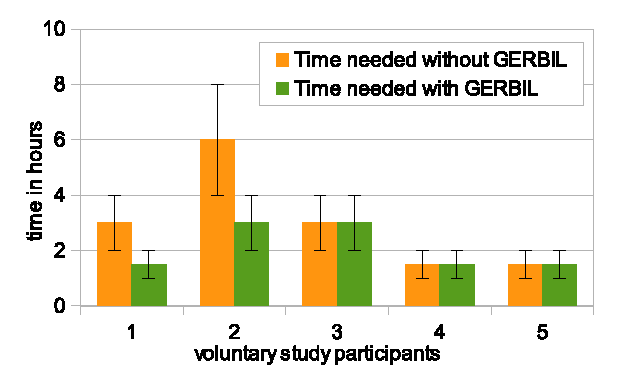
\includegraphics[width=0.48\textwidth]{part_02/benchmarking/ESWC_GERBIL_demo/user_study.eps}
\caption{Comparison of effort needed to implement an adapter for an annotation system.}
\label{cha333:fig:comparedTime}
%\captionof{cha333:figure}{Example spider diagram of recent A2KB experiments with weak annotation matching derived from our online interface.}
\end{figure}

\begin{figure}[ht]
\centering
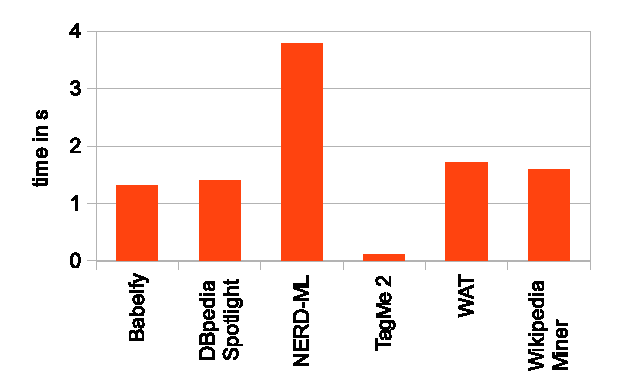
\includegraphics[width=0.48\textwidth]{part_02/benchmarking/ESWC_GERBIL_demo/needed_times.eps}
%\captionof{cha333:figure}{Spider diagram of results of figure \ref{cha333:fig:spiderfmeasure} and their correlation to data set features.}
\caption{Runtime per document for the A2KB experiment type on the MSNBC data set.}
\label{cha333:fig:runtime}
\end{figure}

\begin{comment}
\section{User Interface}
\label{cha333:sec:usecase}
Compliant with the main goal of GERBIL the reproduction of a certain experiment is central to facilitating research efforts. 
Therefore, our web-based platform offers the opportunity to configure an experiment using the parameters defined in Section~\ref{cha333:sec:architecture}.
The results will be displayed as described above and the experiment itself has a time-stamped URL which is citable and will be stable over time smoothing the way to a new citation quality.
Next to individual configurable experiments, GERBIL offers an overview of recent experiment results and correlations to data set features belonging to the same experiment and matching type in the form of a table as well as sophisticated visualizations\footnote{\url{http://gerbil.aksw.org/gerbil/overview}}, see Figure~\ref{cha333:fig:spiderfmeasure} and Figure~\ref{cha333:fig:spiderfeature}.
This allows for a quick comparison of tools and data sets on recently run experiments without additional computational effort.


\todo[inline]{This is a repetition of section 2.}
\textbf{Adding data sets and annotators.}
GERBIL is designed to be extensible, especially w.r.t. novel data sets and entity annotation systems.
Therefore, we differentiate three ways of integrating such data sets.
(1) A user can upload a NIF-based corpus of documents via our web-interface.
(2) GERBIL downloads data sets from \url{datahub.io} which we will then pull via HTTP requests which will be available after manual revision.
(3) Users can also implement a new data set wrapper source code-wise. 
If users than decide to integrate their wrappers intp GERBILs public repository the community will be further-on able to use it for public evaluations.

Additionally, users can submit new webservice-based entity annotation systems in two different ways:
(1) By providing us with the necessary information to call their NIF-based webservice.
Thereby, they need to enter the webservice's URI and a name for the algorithm.
This methods enables fast prototyping of webservices without the need to implement a BAT-framework annotator wrapper.
To lower barriers, we provide a NIF converter in Java.
(2) Additionally, a user can use our source code project, implement a new annotator and push his source code back to us. 
After a feasibility check, we will then bring the enhanced version of GERBIL online and announce it on the website.
Thus, a tremendous gain with respect to possible comparison opportunities in terms of annotators and data sets is inflicted.

GERBIL also provides an opportunity for closed source data\-set evaluation, e.g., business-relevant data or just experimental data not yet ready to be published.
Users can upload their NIF-based data set via GERBILs web interface.
Apart from the experiment results calculated with it, GERBIL will keep \emph{no} other data of such a data set.
\end{comment}

\section{Conclusion and Future Work}
\label{cha333:sec:conclusion}
In this paper, we presented a demo for GERBIL, a platform for the evaluation of annotation frameworks. We presented the different features that make the GERBIL interface easy to use and informative both for end users and developers. 
With GERBIL, we aim to push annotation system developers to better quality and wider use of their frameworks as well as include the provision of persistent URLs for reproducibility and archiving.
%Furthermore, we implemented a generic adaptor for external data sets as well as a generic interface to integrate remote annotator systems.
%The data sets available for evaluation in the previous benchmarking platforms for annotation was extended by \numberOfadditionaldata sets new data sets. Moreover, \numberOfadditionalAnnotators novel annotators were added to the platform. 
%The evaluation of our framework by contributors suggests that adding an annotator to GERBIL demands 1 to 2 hours of work.
%Hence, while keeping the implementation effort previously required to evaluate on a single data set, we allow developers to evaluate on (currently) \overalldata sets times more data sets.
%The presented, web-based frontend allows for several use cases enabling laymen and expert users to perform informed comparisons of semantic annotation tools and spot flaws w.r.t. the used data set features.
%The persistent URIs enhances the long term quotation in the field of information extraction.
%GERBIL is not just a new framework wrapping existing technology. 
%In comparison to earlier frameworks, it 
GERBIL extends the state-of-the-art benchmarks by the capability of considering the influence of NIL attributes and the ability of dealing with data sets and annotators that link to different knowledge bases. In future work, we aim to provide a new theory for evaluating annotation systems and display this information in the GERBIL interface.
%More information about GERBIL and its source code can be found at the project's website. 

%While developing GERBIL, we spotted several flaws in the formal model underlying previous benchmarking frameworks which we aim to tackle in the future. 
%For example, the formal specification underlying current benchmarking frameworks for annotation does not allow using the scores assigned by the annotators for their results. To address this problem, we aim to develop/implement novel measures into GERBIL that make use of scores (e.g., Mean Reciprocal Rank). 
%Moreover, partial results are not considered within the evaluation. For example, during the disambiguation task, named entities without Wikipedia URIs are not considered. This has a significant impact of the number of true and false positives and thus on the performance of some tools.
%Furthermore, certain tasks seem to be too coarse. For example, we will consider splitting the Sa2KB and the A2KB tasks into two subtasks: The first subtask would measure how well tools perform at finding named entities inside the text (NER task) while the second would evaluate how well tools disambiguate those named entities which have been found correctly (similar to the D2KB task).
%Moreover, we plan to provide information about the point in time since when an annotator is stable, i.e., the algorithm underlying the webservice has not changed so as to provide end users with metadata on when to use which annotator.


%\bibliographystyle{abbrv}
%\bibliography{myrefs}


%\end{document}